\chapter{电缆机器人的控制方案设计}\label{chap:control}

由\ref{chap:model}章，我们将整个机器人五连杆腿部结构进行几何分析解算，等效为一根虚拟连杆为虚拟腿，并计算了虚拟腿长、虚拟腿倾角等相关数据。经过虚拟腿的简化，整个机器人模型可以简化为一阶倒立摆模型进行分析控制。
其中机器人底盘及上部结构为倒立摆的“滑块”，腿部结构等效为一根虚拟腿杆件作为“摆杆”，轮腿模型可由此简化为一阶倒立摆模型。

\section{电缆通道检测机器人的简化模型}
\begin{figure}[H]
  \centering
  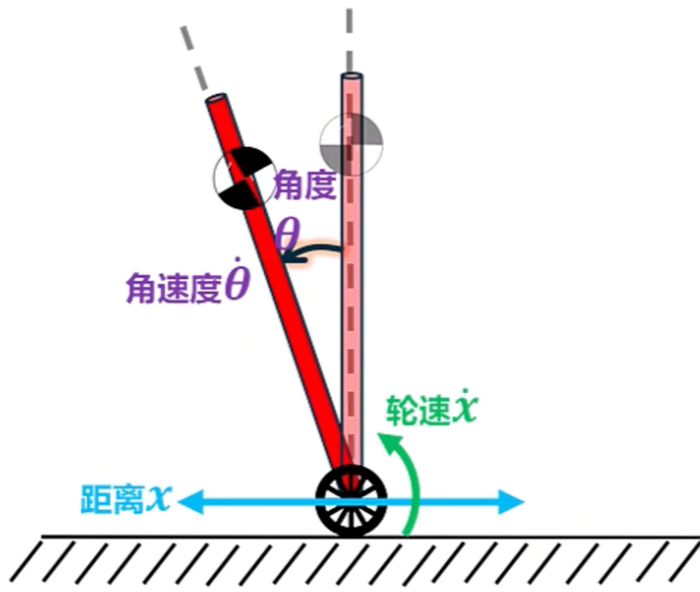
\includegraphics[width=0.5\textwidth]{figures/one_order.png}
  \caption{机器人简化一阶倒立摆示意图}
  \label{fig:one_order}
\end{figure}

\subsection{系统描述与参数定义}
该系统由一个轮子（质量为 $M$）和一个单摆杆（质量为 $m$）组成。我们采用拉格朗日力学法（Lagrange Equation）进行建模。定义系统变量如下：
\begin{table}[H]
  \centering
  \caption{倒立摆参数表}\label{tab:one_order_definition}
  \renewcommand{\arraystretch}{1.3}
  \begin{tabular}{llp{5cm}}
    \toprule
    \textbf{参数} & \textbf{含义}  \\
    \midrule
    $x$ & 轮子中心在水平方向的位移  \\
    $\theta$ & 摆杆相对于垂直向上方向的角度（顺时针为正） \\
    $r$ & 轮子半径 \\
    $h$ & 摆杆质心到旋转轴的距离 \\
    $I$ & 摆杆绕其质心的转动惯量  \\
    $\tau$ & 驱动轮子的电机力矩  \\
    \bottomrule
  \end{tabular}
\end{table}

\subsection{动能与势能分析}
系统的总动能 $T$：
轮子的动能包含平动能与转动能，摆杆的动能由其质心的速度决定。摆杆质心的位置坐标为：
\begin{equation}
  \begin{aligned}
    x_m = x + h\sin\theta \\
    y_m = h\cos\theta
  \end{aligned}
\end{equation}
其速度平方为：
\begin{equation}
v_m^2 = \dot{x}_m^2 + \dot{y}_m^2 = \dot{x}^2 + 2h\dot{x}\dot{\theta}\cos\theta + h^2\dot{\theta}^2
\end{equation}
系统的总动能为：
\begin{equation}
T = \frac{1}{2}(M+m)\dot{x}^2 + \frac{1}{2}(I + mh^2)\dot{\theta}^2 + mh\dot{x}\dot{\theta}\cos\theta
\end{equation}
系统的总势能$V$：
以轮轴为零势能基准面：
\begin{equation}
V = mgh\cos\theta
\end{equation}

\subsection{拉格朗日方程}
定义拉格朗日函数 $L = T - V$。根据拉格朗日方程：
\begin{equation}
\frac{d}{dt}\left(\frac{\partial L}{\partial \dot{q}_i}\right) - \frac{\partial L}{\partial q_i} = Q_i
\end{equation}
其中 $q_i$ 是系统的广义坐标，$Q_i$ 是对应的广义力。对于本系统，选择广义坐标 $q_1 = x$ 和 $q_2 = \theta$，对应的广义力分别为 $Q_1 = \frac{\tau}{r}$（假设轮子与地面之间无滑动）和 $Q_2 = 0$（摆杆不直接受外力矩作用）。通过计算 $\frac{\partial L}{\partial \dot{q}_i}$、$\frac{\partial L}{\partial q_i}$ 和 $\frac{d}{dt}\left(\frac{\partial L}{\partial \dot{q}_i}\right)$，可以得到系统的非线性动力学方程。
其中 $q_1 = x, q_2 = \theta$。对应广义力 $Q_1 = \frac{\tau}{r}$（假设纯滚动），$Q_2 = 0$。
推导得出非线性动力学方程：
\begin{equation}
\begin{cases}
(M + m)\ddot{x} + mh\ddot{\theta}\cos\theta - mh\dot{\theta}^2\sin\theta = \frac{\tau}{r} \\
(I + mh^2)\ddot{\theta} + mh\ddot{x}\cos\theta - mgh\sin\theta = 0
\end{cases}
\end{equation}

\subsection{线性化处理}
在平衡点 $\theta \approx 0$ 附近进行线性化，利用近似条件 $\cos\theta \approx 1, 
\sin\theta \approx \theta, \dot{\theta}^2 \approx 0$：
\begin{equation}
\begin{cases}
(M + m)\ddot{x} + mh\ddot{\theta} = \frac{\tau}{r} \\
mh\ddot{x} + (I + mh^2)\ddot{\theta} - mgh\theta = 0
\end{cases}
\end{equation}

\subsection{状态空间表达式}
令状态向量为 $\mathbf{x} = [\theta, \dot{\theta}, x, \dot{x}]^T$，控制输入 $u = \tau$。联立上述线性方程组，解出 $\ddot{\theta}$ 和 $\ddot{x}$：定义分母行列式：$$D = (M+m)(I+mh^2) - (mh)^2$$整理得到状态空间方程 $\dot{\mathbf{x}} = A\mathbf{x} + Bu$：
\begin{equation}
\begin{bmatrix}
\dot{\theta} \\
\ddot{\theta} \\
\dot{x} \\
\ddot{x}
\end{bmatrix}
=
\begin{bmatrix}
0 & 1 & 0 & 0 \\
\frac{(M+m)mgh}{D} & 0 & 0 & 0 \\
0 & 0 & 0 & 1 \\
-\frac{m^2h^2g}{D} & 0 & 0 & 0
\end{bmatrix}
\begin{bmatrix}
\theta \\
\dot{\theta} \\
x \\
\dot{x}
\end{bmatrix}
+
\begin{bmatrix}
0 \\
-\frac{mh}{Dr} \\
0 \\
\frac{I+mh^2}{Dr}
\end{bmatrix}
\tau
\end{equation}

对于一阶倒立摆（以及更为复杂的轮腿机器人系统），我们通常先证明其开环不稳定但完全可控，进而引入状态反馈（如 LQR 控制器）来实现闭环渐近稳定。以下是为您整理的论文接续内容，您可

\subsection{系统可控性分析}

在设计控制器之前，首先需要判断线性化系统的可控性。对于连续线性时不变系统 $\dot{\mathbf{x}} = A\mathbf{x} + Bu$，其可控性判别矩阵（Controllability Matrix）定义为：
\begin{equation}
Q_c = \begin{bmatrix} B & AB & A^2B & A^3B \end{bmatrix}
\end{equation}

为简化表达，令系统矩阵 $A$ 和输入矩阵 $B$ 中的非零元素分别为：
\begin{equation}
\begin{aligned}
a_{21} &= \frac{(M+m)mgh}{D}, \quad a_{41} = -\frac{m^2h^2g}{D} \\
b_2 &= -\frac{mh}{Dr}, \quad b_4 = \frac{I+mh^2}{Dr}
\end{aligned}
\end{equation}

则矩阵 $A$ 和 $B$ 可简记为：
\begin{equation}
A = \begin{bmatrix} 0 & 1 & 0 & 0 \\ a_{21} & 0 & 0 & 0 \\ 0 & 0 & 0 & 1 \\ a_{41} & 0 & 0 & 0 \end{bmatrix}, \quad B = \begin{bmatrix} 0 \\ b_2 \\ 0 \\ b_4 \end{bmatrix}
\end{equation}

依次计算 $Q_c$ 的各列向量：
\begin{equation}
AB = \begin{bmatrix} b_2 \\ 0 \\ b_4 \\ 0 \end{bmatrix}, \quad A^2B = \begin{bmatrix} 0 \\ a_{21}b_2 \\ 0 \\ a_{41}b_2 \end{bmatrix}, \quad A^3B = \begin{bmatrix} a_{21}b_2 \\ 0 \\ a_{41}b_2 \\ 0 \end{bmatrix}
\end{equation}

由此得到系统的可控性判别矩阵：
\begin{equation}
Q_c = \begin{bmatrix} 0 & b_2 & 0 & a_{21}b_2 \\ b_2 & 0 & a_{21}b_2 & 0 \\ 0 & b_4 & 0 & a_{41}b_2 \\ b_4 & 0 & a_{41}b_2 & 0 \end{bmatrix}
\end{equation}

由于倒立摆系统的物理参数 $M, m, h, I, r$ 均为非零正数，经计算可知该矩阵的行列式 $|Q_c| \neq 0$。因此，可控性矩阵满秩，即 $\text{rank}(Q_c) = 4$。根据卡尔曼秩判据，该一阶倒立摆系统是状态完全可控的，这意味着可以通过设计合适的输入力矩 $\tau$ 来控制系统的所有状态到达期望位置。

\subsection{基于李雅普诺夫理论的稳定性分析}
\subsubsection{开环系统稳定性分析（李雅普诺夫第一方法）}

根据李雅普诺夫间接法（第一方法），线性系统的平衡状态稳定性可由系统矩阵 $A$ 的特征值完全决定。求解矩阵 $A$ 的特征方程：
\begin{equation}
|\lambda I - A| = \begin{vmatrix} \lambda & -1 & 0 & 0 \\ -a_{21} & \lambda & 0 & 0 \\ 0 & 0 & \lambda & -1 \\ -a_{41} & 0 & 0 & \lambda \end{vmatrix} = \lambda^2 (\lambda^2 - a_{21}) = 0
\end{equation}

解得系统的四个开环特征值（极点）为：
\begin{equation}
\lambda_1 = 0, \quad \lambda_2 = 0, \quad \lambda_3 = \sqrt{a_{21}}, \quad \lambda_4 = -\sqrt{a_{21}}
\end{equation}

由于物理参数决定的 $a_{21} = \frac{(M+m)mgh}{D} > 0$，因此 $\lambda_3$ 为正实数。根据李雅普诺夫第一方法，若系统矩阵存在实部大于零的特征值，则该系统在平衡点处是李雅普诺夫不稳定的。这与倒立摆在无控制作用下会自然倾倒的物理直觉相符。

\subsubsection{闭环系统渐近稳定与状态反馈设计（李雅普诺夫第二方法）}
为了使系统稳定在倒立平衡点，需引入状态反馈控制。考虑采用线性二次型调节器（LQR）设计最优控制律：
\begin{equation}
u = -K\mathbf{x}
\end{equation}

其中，$K$ 为状态反馈增益矩阵。此时闭环系统状态方程变为：
\begin{equation}
\dot{\mathbf{x}} = (A - BK)\mathbf{x} = A_{cl}\mathbf{x}
\end{equation}

根据李雅普诺夫直接法（第二方法），构造正定二次型李雅普诺夫函数：
\begin{equation}
V(\mathbf{x}) = \mathbf{x}^T P \mathbf{x}
\end{equation}

其中 $P$ 为对称正定矩阵。对其求时间导数：
\begin{equation}
\dot{V}(\mathbf{x}) = \dot{\mathbf{x}}^T P \mathbf{x} + \mathbf{x}^T P \dot{\mathbf{x}} = \mathbf{x}^T (A_{cl}^T P + P A_{cl}) \mathbf{x}
\end{equation}

为保证系统在平衡点处大范围渐近稳定，要求 $\dot{V}(\mathbf{x})$ 为负定，即存在对称正定矩阵 $Q$，满足连续代数黎卡提方程（CARE）：
\begin{equation}
A_{cl}^T P + P A_{cl} = -Q
\end{equation}

由于系统已证明为完全可控，对于任意给定的半正定状态权重矩阵 $Q$ 和正定控制权重矩阵 $R$，必然存在唯一正定解 $P$，使得通过 $K = R^{-1}B^T P$ 得到的闭环矩阵 $A_{cl}$ 的所有特征值均位于左半复平面。由此，通过 LQR 等状态反馈控制，开环不稳定的倒立摆系统能够被镇定，实现闭环渐近稳定。